\section{Use Cases}

\begin{figure}[H]
    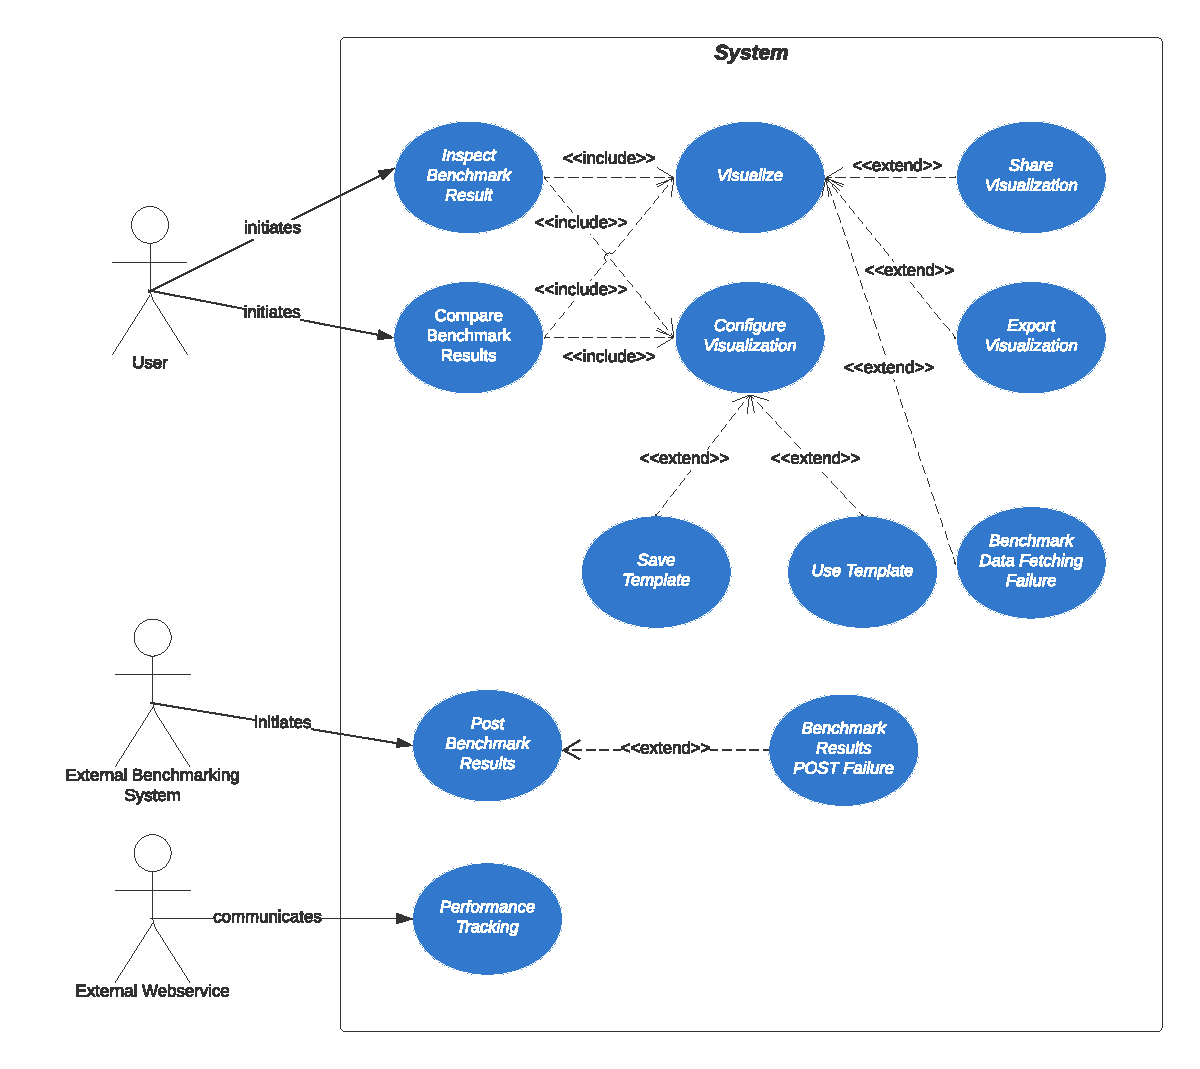
\includegraphics[width=\textwidth]{usecase.pdf}
    \caption{Use case diagram}
    \label{fig:usecase}
\end{figure}

\case{Plot}{cse:plot}
{Generating and displaying a Plot to a User}
{initiated by User}
{\gls{configuration} is available}
{\begin{enumerate}
    \item \parkview{} fetches a \gls{configuration} data from its database.
    \item \parkview{} takes the data and generates the plot specified in the \gls{configuration}.
    \item The user gets redirected to a new site where he can inspect the generated plot.
\end{enumerate}}
{The plot specified by the \gls{configuration} gets shown to the User.}
\implementedby{scn:inspect-last-commit}{cse:plot}
\implementedby{scn:comp-benchmarks}{cse:plot}
\implementedby{scn:fetch-data-failure}{cse:plot}

\bigskip

\case{Configure Plot}{cse:config-vis}
{Configration of a \gls{plot}}
{initiated by User}
{User selected the \enquote{Create New Plot} option}
{\begin{enumerate}
    \item A popup appears.
    \item The user chooses a plot type.
    \item The user chooses between certain options that are specific to the plot type.
\end{enumerate}}
{The \gls{configuration} gets updated.}
\implementedby{scn:inspect-last-commit}{cse:config-vis}
\implementedby{scn:comp-benchmarks}{cse:config-vis}
\implementedby{scn:fetch-data-failure}{cse:config-vis}

\bigskip

\case{Create New Plot}{cse:create-plot}
{Process for configuring and generating a plot}
{initated by User}
{benchmark data for commit is available}
{\begin{enumerate}
    \item The user selects a set of commits.
    \item The user initiates the \texttt{Configure Plot} use case by selecting the \enquote{Create New Plot} option.
    \item Once the user is satisfied with his \gls{configuration}, he initiates the \texttt{Plot} use case by selecting the \enquote{Create New Plot} option in the popup.
\end{enumerate}}
{Plot is displayed to the user}
\implementedby{scn:inspect-last-commit}{cse:create-plot}
\implementedby{scn:comp-benchmarks}{cse:create-plot}

\bigskip

\case{Share Plot}{cse:share-vis}
{Sharing a \gls{plot} using a link}
{initiated by User}
{A \gls{plot} has been generated}
{\begin{enumerate}
    \item The user selects the \enquote{Share Plot} option.
    \item A link gets displayed.
    \item The link redirects any visitors to the same \gls{plot}.
\end{enumerate}}
{A link is shown which redirects to the \gls{plot}}
\implementedby{scn:inspect-last-commit}{cse:share-vis}

\bigskip

\case{Export Plot}{cse:export-vis}
{Downloading a plot}
{initiated by User}
{A \gls{plot} has been generated}
{\begin{enumerate}
    \item The user selects the \enquote{Export Plot} option.
    \item A popup appears.
    \item The user chooses a filetype for the export.
    \item The user confirms and downloads the \gls{plot} in the chosen file format.
\end{enumerate}}
{The User is offered a download of an export of the \gls{plot}}
\implementedby{scn:comp-benchmarks}{cse:export-vis}

\bigskip

\case{Save Template}{cse:save-template}
{Storing a \gls{template} for later use}
{initiated by User}
{The user is in the \texttt{Configure Plot} use case}
{The \texttt{Save Template} use case extends the \texttt{Configure Plot} use case.
\begin{enumerate}
    \item The User selects the \enquote{save template} option.
    \item The User enters a name for the \gls{template}.
    \item \parkview{} stores the template locally for the User (cookies).
\end{enumerate}}
{\Gls{template} is stored locally}
\implementedby{scn:inspect-last-commit}{cse:save-template}

\bigskip

\case{Use Template}{cse:use-temp}
{Using a previously created template}
{initiated by User}
{The user is in the \texttt{Configure Plot} use case and a \gls{template} is available locally}
{The \texttt{Use Template} use case extends the \texttt{Configure Plot} use case.
\begin{enumerate}
    \item The User selects the \enquote{use template} option.
    \item User is shown a list of all available \glspl{template}.
    \item User selects a \gls{template} from the list.
    \item The current \gls{configuration} options get set to the values specified in the template.
\end{enumerate}}
{The \gls{template} is applied to the current configuration.}
\implementedby{scn:comp-benchmarks}{cse:use-temp}

\bigskip

\case{Post Benchmark Results}{cse:post-benchmark-res}
{An external benchmarking system trying to upload benchmark data}
{initiated by External Benchmarking System}
{The external benchmarking system ran the benchmarks}
{\begin{enumerate}
    \item \parkview{} receives a POST request containing benchmark data.
    \item \parkview{} converts the received data into the correct format.
    \item \parkview{} stores the received data in its database.
\end{enumerate}}
{The received performance data is stored in the database}
\implementedby{scn:perf-tracking}{cse:post-benchmark-res}
\implementedby{scn:post-data-failure}{cse:post-benchmark-res}

\bigskip

\case{Performance Tracking}{cse:perf-tracking}
{\parkview{} recognizes big changes in performance and notifies external webservices}
{communicates with External Webservice}
{New benchmark data has been posted to the backend}
{\begin{enumerate}
    \item \parkview{} evaluates the performance of the new benchmark data.
    \item \parkview{} compares the performance of the new benchmark with the performance of the corresponding benchmark of the last commit.
    \item \parkview{} relays the results to a configured number of hooks.
    \item The hooks contact their external webservices according to how they have been configured.
\end{enumerate}}
{\parkview{} fires a POST Request to all webhook subscribers}
\implementedby{scn:inspect-last-commit}{cse:perf-tracking}
\implementedby{scn:perf-tracking}{cse:perf-tracking}

\bigskip

\case{Benchmark Results POST Failure}{cse:benchmark-res-post-fail}
{Behavior in case of invalid POST request}
{communicates with External Benchmarking System}
{The external benchmarking system has sent a POST request}
{This use case extends the \texttt{Post Benchmark Results} use case if an error occurs.
\begin{enumerate}
    \item \parkview{} identifies the error.
    \item \parkview{} creates a response with the correct error code.
\end{enumerate}}
{External Benchmarking System receives a response containing an error code}
\implementedby{scn:post-data-failure}{cse:benchmark-res-post-fail}

\bigskip

\case{Benchmark Data Fetching Failure}{cse:benchmark-data-fetch-fail}
{Behavior in case of invalid request for benchmark data}
{displays error to User}
{This use case extends the \texttt{Plot} use case if an error occurs.}
{\begin{enumerate}
    \item \parkview{} identifies the error.
    \item \parkview{} creates a response with the correct error code.
    \item \parkview{} app displays an error message in the browser.
\end{enumerate}}
{Error message gets displayed}
\implementedby{scn:fetch-data-failure}{cse:benchmark-data-fetch-fail}

